\documentclass[10pt,a4paper]{article}
\usepackage[T1]{fontenc}
\usepackage{amssymb}
\usepackage[left=2.25cm,right=2.25cm,top=2.25cm,bottom=2.75cm]{geometry}
\usepackage{graphicx}
\usepackage{isabelle}
\usepackage{isabellesym}
\usepackage[only,bigsqcap]{stmaryrd}
\usepackage{pdfsetup}

\urlstyle{tt}
\isabellestyle{tt}

\renewcommand{\isacharunderscore}{\_}
\renewcommand{\isachardoublequoteopen}{``}
\renewcommand{\isachardoublequoteclose}{''}

\begin{document}

\title{Stratified Datalog and Program Analysis}
\author{Anders Schlichtkrull, René Rydhof Hansen, Flemming Nielson}
\date{}

\maketitle

\begin{abstract}
\noindent
In this entry we formalize
stratified Datalog, the first such formalization in Isabelle to the best
of our knowledge. Next we formally establish the existence of least
solutions for any stratified Datalog program, essential for reasoning
about negations in clauses. Lastly we illustrate the usefulness of our
Datalog formalization by further formalizing the general Bit-Vector
Framework and formalize and prove correct five analyses in
this framework namely liveness, reaching definitions, available expressions,
very busy expressions and reachability.
Many of our definitions follow Nielson and
Nielson's textbook \cite{DBLP:journals/corr/abs-2012-10086}. 
The formalization is described in our SAC 2024 paper \cite{DBLP:conf/sac/SchlichtkrullHN24}.


\end{abstract}

\tableofcontents

\newpage

% sane default for proof documents
\parindent 0pt
\parskip 0.5ex

\section{Introduction}

In the following we develop the first, to the best of our knowledge,
Isabelle formalization of Datalog in general and stratified Datalog in
particular. We use the formalization to prove the existence of least
solutions (to Datalog programs) with respect to a simple ordering on
predicate valuations. 
The ordering is from Nielson and Nielson's textbook
\cite{NielsonNH:springer1999:PPA}, and appears also
in a paper by Przymusinski \cite{DBLP:books/mk/minker88/Przymusinski88} in a different formulation.
We prove the two formulations equivalent.
Furthermore, we apply our formalization to also
formalize so-called \emph{bit-vector
  analyses}~\cite{NielsonNH:springer1999:PPA} as Datalog programs
covering all the usual
variants~\cite{DBLP:journals/corr/abs-2012-10086}: forward may
analyses, backward may analyses, forward must analyses, and backward
must analyses. The analyses are proved to correctly summarize the
paths in the program, and we additionally show that each variant of
our Bit-Vector Framework has an instance by formalizing four classic
analyses: reaching definitions, live variables, available expressions,
and very busy expressions~\cite{NielsonNH:springer1999:PPA}.
We use the labeled transition systems formalization
by Schlichtkrull et al.~\cite{Labeled_Transition_Systems-AFP,DBLP:conf/fmcad/SchlichtkrullSST22} to represent program graphs.

A Rocq formalization of stratified Datalog, based on the thesis by
Dumbrava~\cite{DBLP:phd/hal/Dumbrava16}, has been developed by
Benzaken et al.~\cite{DBLP:conf/itp/BenzakenCD17}, giving a
comprehensive formalization focusing on correctness of evaluation
strategies for (stratified) Datalog programs. 

Non-stratified Datalog has been independently formalized in Rocq 
for use as a stepping stone for formalizing further logics (Binder,
Horn clauses, BCiC) used to model and reason about authentication~\cite{DBLP:conf/types/Whitehead06} and a subset called Regular Datalog has also been formalized in Rocq~\cite{DBLP:journals/tplp/BonifatiDA18}.
Rocq has also been used to
formalize various semantics for Prolog (with corresponding proofs of
equivalence), with the goal of proving correctness of
static analyses of Prolog programs~\cite{DBLP:conf/ppdp/KrienerKB13}.
Non-stratified Datalog has also been formalized in
Lean with the goal of certifying results from Datalog reasoners \cite{TGMK2025}.

Formalizations of analysis frameworks and the underlying theory have
mainly focused on the \emph{abstract
  interpretation}~\cite{DBLP:conf/popl/CousotC77} approach to static
analysis and primarily using Rocq, with impressive
results~\cite{DBLP:conf/itp/CacheraP10,DBLP:conf/popl/JourdanLBLP15}.
Additionally an Isabelle formalization of abstract interpretation
of a small imperative language occurs in the ``fully mechanized'' semantics
textbook of
Nipkow~\cite{DBLP:books/sp/NipkowK14,DBLP:conf/itp/Nipkow12}.

Concrete program analyses have been formalized and proven correct in
Isabelle, as witnessed in the Archive of Formal
Proofs\footnote{\url{https://www.isa-afp.org/topics/computer-science/programming-languages/static-analysis/}},
including slicing, control flow analysis, conflict analysis, call
arity analysis
etc.~\cite{Program-Conflict-Analysis-AFP,Slicing-AFP,DBLP:phd/dnb/Breitner16,HRB-Slicing-AFP,Shivers-CFA-AFP,DBLP:conf/sas/LammichM08,RIPEMD-160-SPARK-AFP,Call_Arity-AFP,Dominance_CHK-AFP,DBLP:conf/tphol/WasserrabL08,DBLP:conf/pldi/WasserrabLS09}.
These do not use Datalog.

\begin{figure}
\begin{center}
  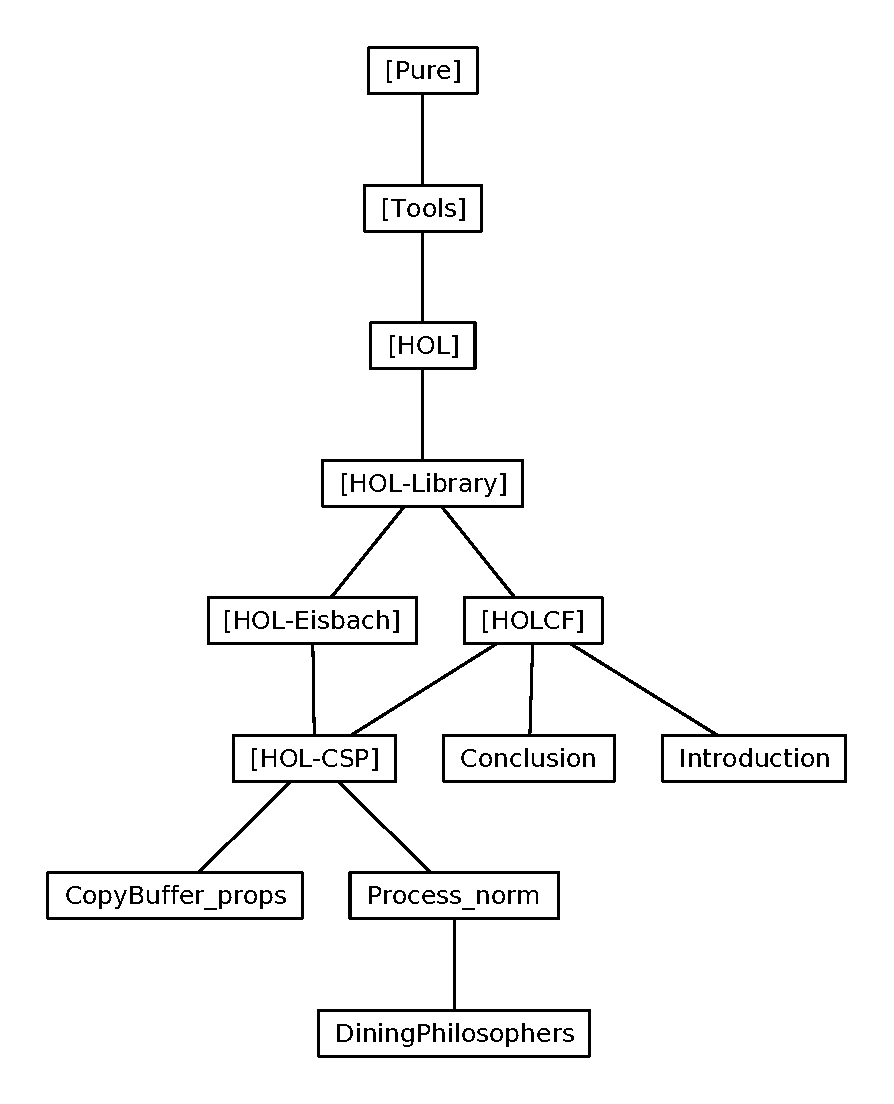
\includegraphics[width=0.7\textwidth,keepaspectratio]{session_graph}
\end{center}
\caption{Theory dependency graph}
\label{fig:thys}
\end{figure}

\newpage

% generated text of all theories
\input{session}

% optional bibliography
\bibliographystyle{alpha}
\bibliography{root}

\end{document}
\endinput
